\section{Higher Dimensional Manifolds}

\subsection{Lemmas}
\begin{lem}
\label{lem:manifolds_0}
If \(\DConf_n(\Gamma)\) is an \(m\)-manifold with or without boundary, 
then \(\Gamma\) has at least \(n+m\) vertices and \(n \ge m\).
\end{lem}
\begin{proof}
    If \(\Gamma\) has less than \(n\) vertices, then \(\DConf_n(\Gamma)\) is empty;
    so, suppose \(\Gamma\) has at least \(n\) vertices.
    If \(\Gamma\) has less than \(n + m\) vertices, then
    for any configuration of \(n\) particles on \(\Gamma\)
    at most \(m-1\) particles can simultaneously move.
    Since exactly \(m\) particles need to be able to simultaneously move for an \(m\)-cube 
    to exist in \(\DConf_n(\Gamma)\), no configuration in \(\DConf_n(\Gamma)\)
    can have a neighborhood homeomorphic to an open set in \(\mathbb{R}^m\).

    Similarly, if \(n < m\), then there are not enough particles that can simultaneously move
    for an \(m\)-cube to exist in \(\DConf_n(\Gamma)\). So, \(n \ge m\). 
\end{proof}

Suppose \(\Conf_n(\Gamma)\) is an \(m\)-manifold without boundary and \(n \ge 3\).
By Lemma \ref{lem:manifolds_0}, \(\Gamma\) must have at least \(n + m \ge 2m\) vertices.
Let \(\{v_{\alpha} w_{\alpha}\}_{\alpha=1}^{m-1}\) be a collection of \(m-1\) disjoint edges in \(\Gamma\).
We write \(\Gamma - \{v_\alpha, w_\alpha\}_{\alpha=1}^{m-1}\) to mean the subgraph of \(\Gamma\)
obtained after removing the vertices \(\{v_\alpha, w_\alpha\}_{\alpha=1}^{m-1}\) from \(\Gamma\).
Notice that \(\Gamma - \{v_\alpha, w_\alpha\}_{\alpha=1}^{m-1}\) has at least \(n + m - 2(m-1) = n - m + 2\) vertices.


\begin{lem}
    \label{lem:manifolds_1}
    For any collection of \(n - m + 1\) vertices \(\{v_\alpha\}_{\alpha=m}^n\)
    in \(\Gamma - \{v_\alpha,  w_\alpha\}_{\alpha=1}^{m-1}\), there exists exactly two edges
    \(e_1 = v_i u_1\) and \(e_2 = v_j u_2\) such that
    \begin{enumerate}[label=(\roman*)]
    \item \(m \leq i, j \leq n\)
    \item \(u_1, u_2 \not \in \{v_\alpha\}_{\alpha=1}^n\cup\{w_\alpha\}_{\alpha=1}^{m-1}\)
    \item Exactly one of the following hold in Figure \ref{fig:lem:manifolds_1}
    \end{enumerate}
    \begin{figure}[h!]
        \centering
        \begin{enumerate*}[label=(\arabic*)]
            \item \label{fig:lem:manifolds_1_1}
            \begin{minipage}{.3\textwidth}
                \centering
                \(v_i = v_j\) \textit{and} \(u_1 \neq u_2\) \\
                \vspace{1em}
                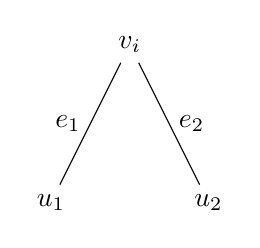
\begin{tikzpicture}
                    \node (vi) at (3, 2) {\(v_i\)};
                    \node (w2) at (2, 0) {\(u_1\)};
                    \node (w3) at (4, 0) {\(u_2\)};

                    \draw (vi) -- (w2) node[midway, left] {\(e_1\)};
                    \draw (vi) -- (w3) node[midway, right] {\(e_2\)};
                \end{tikzpicture} 
            \end{minipage}

            \hspace{3em}

            \item \label{fig:lem:manifolds_1_2}
            \begin{minipage}{.3\textwidth}
                \centering
                \(u_1 = u_2\) \textit{and} \(v_i \neq v_j\) \\
                \vspace{1em}
                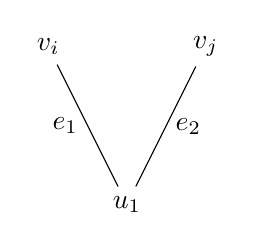
\begin{tikzpicture}
                    \node (vi) at (2, 2) {\(v_i\)};
                    \node (vj) at (4, 2) {\(v_j\)};
                    \node (w2) at (3, 0) {\(u_1\)};

                    \draw (vi) -- (w2) node[midway, left] {\(e_1\)};
                    \draw (vj) -- (w2) node[midway, right] {\(e_2\)};
                \end{tikzpicture}
            \end{minipage}
        \end{enumerate*}
        \caption{Lemma \ref{lem:manifolds_1} possibilities.}
        \label{fig:lem:manifolds_1}
    \end{figure}
\end{lem}

\begin{proof}
    Let \(\{v_\alpha\}_{\alpha=m}^n\) be a collection of \(n - m + 1\) vertices in \(\Gamma - \{v_\alpha, w_\alpha\}_{\alpha=1}^{m-1}\)
    and put a particle at each vertex in \(\{v_\alpha\}_{\alpha=1}^n\).
    The movements of the particles from \((v_\alpha)_{\alpha=1}^{m-1}\) to \((w_\alpha)_{\alpha=1}^{m-1}\)
    correspond to an \((m-1)\)-cube in \(\DConf_n(\Gamma)\).
    Since the configuration space is an \(m\)-manifold without boundary, 
    this \((m-1)\)-cube must border exactly two distinct \(m\)-cubes.
    For this \((m-1)\)-cube to border two \(m\)-cubes,
    there needs to exist two additional mutually exclusive particle movements.
    Let \(v_i, v_j \in \{v_\alpha\}_{\alpha=m}^n\) be the vertices that these particles occupy.
    Since the particle(s) at \(v_i\) and \(v_j\) need to move simultaneously as the particles move from \((v_\alpha)_{\alpha=1}^{m-1}\) to \((w_\alpha)_{\alpha=1}^{m-1}\),
    there exist destination(s) \(u_1\) and \(u_2\) outside the set \(\{v_{\alpha}\}_{\alpha=1}^n \cup \{w_\alpha\}_{\alpha=1}^{m-1}\).
    In order for these additional movements to be mutually exclusive, either \(v_i \neq v_j\) or \(u_1 \neq u_2\) but not both.
\end{proof}

\begin{rem}
If \(\Gamma - \{v_\alpha, w_\alpha\}_{\alpha=1}^{m-1}\) has exactly \(n - m + 2\) vertices,
then only case \ref{fig:lem:manifolds_1_2} in can occur.
\end{rem}

\subsection{A painful and long lemma}
\begin{lem}
    \label{lem:manifolds_2}
    Let \(\{v_\alpha\}_{\alpha=m}^{n}\) be a collection of \(n-m+1\) vertices in 
    \(\Gamma - \{v_\alpha w_\alpha\}_{\alpha=1}^{m-1}\).
The edges \(e_1\) and \(e_2\) guaranteed from applying Lemma \ref{lem:manifolds_1} 
to \(\{v_\alpha\}_{i=m}^{n}\) in the graph \(\Gamma - \{v_\alpha w_\alpha\}_{i=\alpha}^{m-1}\) satisfy exactly one of the following:
\begin{enumerate}[label=(\roman*)]
        \item \(n = m+1\) and these edges belong to a \(Y\)-graph in \(\Gamma - \{v_i, w_i\}_{i=1}^{m-1}\) with two vertices not in \(\{v_i\}_{i=1}^n\).
        \item \(e_1\) and \(e_2\) belong to a \(3\)-cycle in \(\Gamma - \{v_i, w_i\}_{i=1}^{m-1}\) with exactly two vertices not in \(\{v_i\}_{i=1}^n\).
        \item \(e_1\) and \(e_2\) belong to an \(r\)-cycle in \(\Gamma - \{v_i, w_i\}_{i=1}^{m-1}\) with exactly one vertex not in \(\{v_i\}_{i=1}^n\) and \(3 \le r \le (n-m)+2\).
\end{enumerate}

\end{lem}


\begin{proof}
    The argument proceeds by cases on the possibilities for the edges \(e_1\) and \(e_2\).
    
    \textbf{Case 1:} \(v_i = v_j\) and \(u_1 \neq u_2\) (See case \ref{fig:lem:manifolds_1_1} in Figure \ref{fig:lem:manifolds_1}). 
    In this case, \(e_1 = v_i u_1\) and \(e_2 = v_i u_2\). 
    Let \(v_k\) be some vertex in \(\{v_\alpha\}_{i=m}^n\setminus\{v_i\}\).
    Applying Lemma \ref{lem:manifolds_1} to \(\{u_1\}\cup\{v_\alpha\}_{\alpha=m}^n\setminus\{v_k\}\) in \(\Gamma - \{v_\alpha, w_\alpha\}_{\alpha=1}^{m-1}\),
    we obtain two new edges \(e_3\) and \(e_4\).
    Since \(e_2\) already connects \(v_i\) to \(u_2\) and there must be exactly two edges
    with exactly one endpoint in \(\{u_1\}\cup\{v_\alpha\}_{\alpha=m}^n\setminus\{v_k\}\),
    one of \(e_3\) or \(e_4\) is \(e_2\). 
    Without a loss of generality suppose \(e_4 = e_2\).
    Since \(e_3\) must share an endpoint with \(e_4 = e_2\), it follows that \(e_3\) has either \(v_i\) as an endpoint or \(u_2\) as an endpoint (See Figure \ref{fig:lem:is_surface_2_0}).
    \begin{figure}[h!]
        \centering
        \begin{tikzpicture}
            \node (v1) at (0,2) {\(v_1\)};
            \node (w1) at (0,0) {\(w_1\)};
            \draw (v1) -- (w1);
            \node (vi) at (3, 2) {\(v_i\)};
            \node (w2) at (2, 0) {\(w_2\)};
            \node (w3) at (4, 0) {\(w_3\)};
            \draw (vi) -- (w2) node[midway, left] {\(e_1\)};
            \draw (vi) -- (w3) node[midway, right] {\(e_2\)};
            
            \node (vk) at (5, 2) {\(?\)};
            \draw (vi) -- (vk) node[midway, above] {\(e_3\)};
        \end{tikzpicture}
        \quad\quad
        \begin{tikzpicture}
            \node (v1) at (0,2) {\(v_1\)};
            \node (w1) at (0,0) {\(w_1\)};
            \draw (v1) -- (w1);
            \node (vi) at (3, 2) {\(v_i\)};
            \node (w2) at (2, 0) {\(w_2\)};
            \node (w3) at (4, 0) {\(w_3\)};
            \node (q) at (6, 0) {\(?\)};
            \draw (vi) -- (w2) node[midway, left] {\(e_1\)};
            \draw (vi) -- (w3) node[midway, right] {\(e_2\)};
            \draw (q) -- (w3) node[midway, below] {\(e_3\)};
            
        \end{tikzpicture}
        \caption{Possibilities if \(v_i = v_j\)}
        \label{fig:lem:is_surface_2_0}
    \end{figure}

    Lemma \ref{lem:manifolds_1} guarantees relevant two facts about the edges \(e_1\), \(e_2\), and \(e_3 = e_4\).
    % TODO continue fixing from here.
    \begin{enumerate}
        \item \(e_1\) and \(e_2\) are the only edges with exactly one endpoint in \(\{v_\alpha\}_{\alpha=1}^{m-1}\).
        \item \(e_3\) and \(e_4 = e_2\) are the only edges with exactly one endpoint in \(\{w_2, v_2, \cdots, v_n\}\setminus\{v_k\}\).
    \end{enumerate}
    We claim that if \(e_3\) has \(v_i\) as an endpoint, then \(v_k\) must be the other endpoint of \(e_3\)
    (see the graph on the left in Figure \ref{fig:lem:is_surface_2_1}).
    To verify this claim, suppose \(e_3\) has \(v_i\) as an endpoint and let \(v^*\) be the other endpoint of \(e_3\).
    Since \(e_3 \neq e_1\) and \(e_3 \neq e_2\) but \(e_3\) has \(v_i\) as an endpoint, the first fact above 
    guarantees that \(v^* \in \{v_2, \cdots, v_n\}\).
    The second fact guarantees that \(v^* \not \in \{w_2, v_2, \cdots, v_n\}\setminus\{v_k\}\).
    Hence,
    \[
        v^* \in \left(V(\Gamma - \{v_1, w_1\})\setminus(\{w_2, v_2, \cdots, v_n\}\setminus\{v_k\})\right) \cap \{v_2, \cdots, v_n\} = \{v_k\}.
    \]

    Moreover, if \(e_3\) has \(v_i\) as an endpoint, 
    then since \(v_k\) was arbitrary, 
    every vertex in \(\{v_2, \cdots, v_n\}\setminus\{v_i\}\) is adjacent to \(v_i\).

    So, if \(n > 3\) then there are two vertices say \(v_k\) and \(v_r\) in the set \(\{v_2, \cdots, v_n\}\) that are distinct but adjacent to \(v_i\).
    Put particles at each vertex in the set \(\{w_2, v_1, \cdots, v_n\}\setminus\{v_i\}\).
    As the particle at \(v_1\) moves to \(w_1\), any one particle in the set \(\{w_2, v_k, v_r\}\) can move to \(v_i\).
    These particles movements result in a book in the configuration space whose spine corresponds to the movement of the particle at \(v_1\) to \(w_1\).
    Therefore if \(e_3\) has \(v_i\) as an endpoint, then \(e_1\) and \(e_2\) belong to a \(Y\)-graph \textit{and} \(n = 3\).

    \begin{figure}[h!]
        \centering
        \begin{tikzpicture}
            \node (v1) at (0,2) {\(v_1\)};
            \node (w1) at (0,0) {\(w_1\)};
            \draw (v1) -- (w1);
            \node (vi) at (3, 2) {\(v_i\)};
            \node (w2) at (2, 0) {\(w_2\)};
            \node (w3) at (4, 0) {\(w_3\)};
            \draw (vi) -- (w2) node[midway, left] {\(e_1\)};
            \draw (vi) -- (w3) node[midway, right] {\(e_2\)};
            
            \node (vk) at (5, 2) {\(v_k\)};
            \draw (vi) -- (vk) node[midway, above] {\(e_3\)};
        \end{tikzpicture}
        \quad\quad
        \begin{tikzpicture}
            \node (v1) at (0,2) {\(v_1\)};
            \node (w1) at (0,0) {\(w_1\)};
            \draw (v1) -- (w1);
            \node (vi) at (3, 2) {\(v_i\)};
            \node (w2) at (2, 0) {\(w_2\)};
            \node (w3) at (4, 0) {\(w_3\)};
            \draw (vi) -- (w2) node[midway, left] {\(e_1\)};
            \draw (vi) -- (w3) node[midway, right] {\(e_2\)};
            \draw (w2) -- (w3) node[midway, below] {\(e_3\)};
            
        \end{tikzpicture}
        \caption{Possibilities if \(v_i = v_j\)}
        \label{fig:lem:is_surface_2_1}
    \end{figure}

    Suppose now that \(e_3\) has \(w_3\) as an endpoint.
    We claim that \(e_3\) must have \(w_2\) as its other endpoint
    (see the graph on the right in Figure \ref{fig:lem:is_surface_2_1}).
    To verify this claim, let \(w_*\) be the other endpoint of \(e_3\).
    Since \(w_3 \not \in \{w_2, v_2, \cdots, v_n\}\setminus\{v_k\}\),
    the second fact above guarantees that \(w_*\) must belong to \(\{w_2, v_2, \cdots, v_n\}\setminus\{v_k\}\).
    Since \(e_3 \neq e_1\) and \(e_3 \neq e_2\), the first fact above guarantees that \(w_*\)
    cannot belong to \(\{v_2, \cdots, v_n\}\).
    The only possibility left is that \(w_* = w_2\).

    Therefore, if \(e_3\) has \(w_3\) as an endpoint, then \(e_1\) and \(e_2\) belong to a \(3\)-cycle with two vertices
    not in \(\{v_2, \cdots, v_n\}\).

    \textbf{Case 2:} \(v_i \neq v_j\) (See \ref{fig:lem:is_surface_1_1:2} in Figure \ref{fig:lem:is_surface_1_1}).
    In this case, \(e_1 = v_i w_2\) and \(e_2 = v_j w_2\).
    Applying Lemma \ref{lem:is_surface_1} to \(\{w_2, v_2, \cdots, v_n\}\setminus\{v_j\}\) in \(\Gamma - \{v_1, w_1\}\),
    we again obtain two edges \(e_3\) and \(e_4\).
    Since \(e_2\) already connects \(v_j\) to \(w_2\)
    and there must be exactly two edges with exactly one endpoint in \(\{w_2, v_2, \cdots, v_n\}\setminus\{v_j\}\), 
    one of \(e_3\) or \(e_4\) is \(e_2\).
    Without a loss of generality suppose \(e_4 = e_2\).
    Since \(e_3\) must share an endpoint with \(e_4 = e_2\), it follows that \(e_3\)
    has either \(w_2\) or \(v_j\) as an endpoint
    (see Figure \ref{fig:lem:is_surface_2_2}).
    \begin{figure}[h!]
        \centering
        \begin{tikzpicture}
            \node (v1) at (0,2) {\(v_1\)};
            \node (w1) at (0,0) {\(w_1\)};
            \draw (v1) -- (w1);
            \node (vi) at (2, 2) {\(v_i\)};
            \node (vj) at (4, 2) {\(v_j\)};
            \node (w2) at (3, 0) {\(w_2\)};
            \draw (vi) -- (w2) node[midway, left] {\(e_1\)};
            \draw (vj) -- (w2) node[midway, right] {\(e_2\)};

            \node (q) at (5, 0) {\(?\)};
            \draw (w2) -- (q) node[midway, below] {\(e_3\)};
        \end{tikzpicture}
        \quad\quad
        \begin{tikzpicture}
            \node (v1) at (0,2) {\(v_1\)};
            \node (w1) at (0,0) {\(w_1\)};
            \draw (v1) -- (w1);
            \node (vi) at (2, 2) {\(v_i\)};
            \node (vj) at (4, 2) {\(v_j\)};
            \node (w2) at (3, 0) {\(w_2\)};
            \draw (vi) -- (w2) node[midway, left] {\(e_1\)};
            \draw (vj) -- (w2) node[midway, right] {\(e_2\)};

            \node (q) at (6, 2) {\(?\)};
            \draw (vj) -- (q) node[midway, above] {\(e_3\)};
        \end{tikzpicture}
        \caption{Possibilities if \(v_i \neq v_j\)}
        \label{fig:lem:is_surface_2_2}
    \end{figure}

    Since \(e_1\) and \(e_2\) are the only edges connecting a vertex in \(\{v_2, \cdots, v_n\}\) to \(w_2\) and \(e_3 \neq e_1\) and \(e_3 \neq e_2\),
    if \(e_3\) has \(w_2\) as endpoint, then \(e_3\) must connect \(w_2\) to some vertex \(w_3\) in \(\Gamma - \{v_1, w_1\}\) outside the set \(\{v_2, \cdots, v_n\}\).

    Suppose that \(e_3\) has \(w_2\) but \(n > 3\),
    then there exists some \(v_k\) in \(\{v_2, \cdots, v_n\}\) distinct from \(v_i\) and \(v_j\). 
    Let \(w_3\) be the other endpoint of \(e_3\) as before and put particles at the vertices \(\{w_3, v_1, \cdots, v_n\}\setminus\{v_k\}\). 
    As the particle at \(v_1\) moves to \(w_1\),
    any one particle in the set \(\{v_i, v_j, w_3\}\) can move to \(w_2\). 
    These particles movements results in a book in the configuration space whose spine corresponds to the movement of the particle at \(v_1\) to \(w_1\). 
    Hence, if \(e_3\) has \(w_2\) as an endpoint, 
    then \(n=3\) \textit{and} \(e_1\) and \(e_2\) both belong to a \(Y\)-graph with two vertices not in \(\{v_2, \cdots, v_n\}\)
    (see the graph on the left in Figure \ref{fig:lem:is_surface_2_3}).

    \begin{figure}[h!]
        \centering
        \begin{tikzpicture}
            \node (v1) at (0,2) {\(v_1\)};
            \node (w1) at (0,0) {\(w_1\)};
            \draw (v1) -- (w1);
            \node (vi) at (2, 2) {\(v_i\)};
            \node (vj) at (4, 2) {\(v_j\)};
            \node (w2) at (3, 0) {\(w_2\)};
            \draw (vi) -- (w2) node[midway, left] {\(e_1\)};
            \draw (vj) -- (w2) node[midway, right] {\(e_2\)};

            \node (u) at (5, 0) {\(w_3\)};
            \draw (w2) -- (u) node[midway, below] {\(e_3\)};
        \end{tikzpicture}
        \quad\quad
        \begin{tikzpicture}
            \node (v1) at (0,2) {\(v_1\)};
            \node (w1) at (0,0) {\(w_1\)};
            \draw (v1) -- (w1);
            \node (vi) at (2, 2) {\(v_i\)};
            \node (vj) at (4, 2) {\(v_j\)};
            \node (w2) at (3, 0) {\(w_2\)};
            \draw (vi) -- (w2) node[midway, left] {\(e_1\)};
            \draw (vj) -- (w2) node[midway, right] {\(e_2\)};

            \node (vk) at (6, 2) {\(v_k\)};
            \draw (vk) -- (vj) node[midway, above] {\(e_3\)};
        \end{tikzpicture}
        \caption{Possibilities if \(v_i \neq v_j\)}
        \label{fig:lem:is_surface_2_3}
    \end{figure}

    Finally, suppose that \(e_3\) has \(v_j\) as an endpoint. 
    Since \(e_1\) and \(e_2\) are the only edges with exactly one endpoint in \(\{v_2, \cdots, v_n\}\),
    the other endpoint of \(e_3\) must belong to \(\{v_2, \cdots, v_n\}\setminus\{v_j\}\).
    Let \(v_k\) be this endpoint and notice that \(\{v_i, w_2, v_j, v_k\}\) cannot belong to a \(Y\)-graph
    (see the graph on the right in Figure \ref{fig:lem:is_surface_2_3}).
    
    We claim that the vertices in \(\{v_i, w_2, v_j, v_k\}\) belong to a cycle.
    If \(n = 3\), the only possible choice for \(v_k\) is \(v_i\), 
    meaning the vertices in \(\{w_2, v_2, v_3\}\) form a \(3\)-cycle in \(\Gamma - \{v_1, w_1\}\).
    So suppose \(n > 3\) and relabel the vertices in \(\{v_i, w_2, v_j, v_k\}\) such that 
    \(v_i = u_1, w_2 = u_2, v_j = u_3, v_k = u_4\) (see Figure \ref{fig:lem:is_surface_2_4}).
    \begin{figure}[h!]
        \centering
        \begin{tikzpicture}
            \node (v1) at (0,2) {\(v_1\)};
            \node (w1) at (0,0) {\(w_1\)};
            \draw (v1) -- (w1);

            \node (u1) at (2, 1) {\(u_1\)};
            \node (u2) at (3, 0) {\(u_2\)};
            \node (u3) at (4, 1) {\(u_3\)};
            \node (u4) at (3, 2) {\(u_4\)};
            \draw (u1) -- (u2) node[midway, below left] {\(e_1\)};
            \draw (u2) -- (u3) node[midway, below right] {\(e_2\)};
            \draw (u3) -- (u4) node[midway, above right] {\(e_3\)};
        \end{tikzpicture}
        \caption{Partial cycle if \(v_i \neq v_j\) and \(e_3\) has \(v_j\) as an endpoint.}
        \label{fig:lem:is_surface_2_4}
    \end{figure}

    We now inductively construct a path in \(\Gamma\)
    consisting of vertices in \(\{w_2, v_2, \cdots, v_n\}\) starting at \(u_1\).

    Suppose \(u_{i-1}, u_i, u_{i+1}\) are 3 distinct vertices in \(\{w_2, v_2, \cdots, v_n\}\) such that
    \(u_{i-1}\) is connected to \(u_{i-2}\) by the edge \(e_{i-2}\)
    and \(u_i\) is connected to \(u_{i-1}\) by the edge \(e_{i-1}\) for some \(i > 3\).
    Apply Lemma \ref{lem:is_surface_1} to \(\{w_2, v_2, \cdots, v_n\}\setminus\{u_i\}\) in \(\Gamma - \{v_1, w_1\}\) and obtain
    two edges \(e\) and \(e'\).
    Since \(e\) and \(e'\) are 
    the only edges with exactly one endpoint in \(\{w_2, v_2, \cdots, v_n\}\setminus\{u_i\}\)
    and  \(u_i\) is already adjacent to \(u_{i-1}\), one of \(e\) or \(e'\) must
    be the edge \(e_{i-1}\).
    Without a loss of generality suppose \(e' = e_{i-1}\) and define \(e_i = e\).

    Since \(e_{i-1}\) and \(e_{i}\) must share an endpoint,
    one of the endpoints of \(e_i\) is \(u_{i-1}\) or \(u_i\). 
    Let \(u_*\) be the other endpoint of \(e_i\) (see Figure \ref{fig:lem:is_surface_2_5}).

    \begin{figure}[h!]
        \centering
        \begin{tikzpicture}
            \node (v1) at (0,2) {\(v_1\)};
            \node (w1) at (0,0) {\(w_1\)};
            \draw (v1) -- (w1);
            \node (u1) at (2, 2) {\(u_{i-2}\)};
            \node (u2) at (3, 0) {\(u_{i-1}\)};
            \node (u3) at (4, 2) {\(u_{i}\)};
            \draw (u1) -- (u2) node[midway, left] {\(e_{i-2}\)};
            \draw (u2) -- (u3) node[midway, right] {\(e_{i-1}\)};

            \node (q) at (5, 0) {\(u_*\)};
            \draw (u2) -- (q) node[midway, below] {\(e_i\)};
        \end{tikzpicture}
        \quad\quad
        \begin{tikzpicture}
            \node (v1) at (0,2) {\(v_1\)};
            \node (w1) at (0,0) {\(w_1\)};
            \draw (v1) -- (w1);
            \node (u1) at (2, 2) {\(u_{i-2}\)};
            \node (u2) at (3, 0) {\(u_{i-1}\)};
            \node (u3) at (4, 2) {\(u_{i}\)};
            \draw (u1) -- (u2) node[midway, left] {\(e_{i-2}\)}; 
            \draw (u2) -- (u3) node[midway, right] {\(e_{i-1}\)};

            \node (q) at (6, 2) {\(u_*\)};
            \draw (u3) -- (q) node[midway, above] {\(e_i\)};
        \end{tikzpicture}
        \caption{Possibilities for \(e_i\)}
        \label{fig:lem:is_surface_2_5}
    \end{figure}

    Suppose \(e_i\) has \(u_{i-1}\) as an endpoint.
    Since \(e_i\) cannot share both its endpoints with \(e_{i-1}\), and
    \(e_i\) has exactly one endpoint in \(\{w_2, v_2, \cdots, v_n\}\setminus\{u_i\}\),
    it follows that \(u_*\) must fall outside of \(\{w_2, v_2, \cdots, v_n\}\).
    Put particles at each vertex in the set \(\{u_*, w_2, v_1, v_2, \cdots, v_n\}\setminus\{u_{i-2}, u_i\}\).
    Since \(i > 3\), as the particle at \(v_1\) travels to \(w_1\),
    the particle at \(u_{i-3}\) can travel to \(u_{i-2}\) simultaneously as the particle
    at \(u_{i-1}\) can travel to \(u_i\).
    These particles movements result in a \(3\)-cube in the configuration space.
    Therefore \(e_i\) cannot have \(u_{i-1}\) as an endpoint.
    
    Suppose instead that \(e_i\) has \(u_i\) as an endpoint.
    Since \(e_i\) must have exactly one endpoint in \(\{w_2, v_2, \cdots, v_n\}\setminus\{u_i\}\) and \(u_* \neq u_i\),
    it follows that \(u_*\) must belong to \(\{w_2, v_2, \cdots, v_n\}\setminus\{u_i, u_{i-1}\}\).
    Define \(u_{i+1} = u_*\).
    This completes the inductive step.
    
    Notice that each \(u_i\) belongs to the finite set \(\{w_2, v_2, \cdots, v_n\}\)
    and \(u_i\) is connected to \(u_{i-1}\) by the edge \(e_{i-1}\) for all \(i > 1\).
    We claim this path must eventually return to \(u_1\) forming a cycle.

    Let \(r\) be the largest integer such that \(u_r \not \in \{u_1, \cdots, u_{r-1}\}\).
    The edge \(e_r\) must connect \(u_r\) to some vertex \(u_k \in \{u_1, \cdots, u_{r-1}\}\)
    otherwise we contradict that \(r\) is maximal.
    Suppose \(k > 1\), then \(e_{k-1}\), \(e_k\), and \(e_r\) are three distinct
    edges sharing \(u_k\) as a common endpoint (see Figure \ref{fig:lem:is_surface_2_6}).

    \begin{figure}[h!]
        \centering
        \begin{tikzpicture}
            \node (ukm1) at (0,0) {\(u_{k-1}\)};
            \node (uk) at (2,0) {\(u_k\)};
            \node (ukp1) at (4,0) {\(u_{k+1}\)};
            \node (um) at (2,2) {\(u_r\)};

            \draw (ukm1) -- (uk) node[midway, below] {\(e_{k-1}\)};
            \draw (uk) -- (ukp1) node[midway, below] {\(e_k\)};
            \draw (uk) -- (um) node[midway, left] {\(e_r\)};
        \end{tikzpicture}
        \caption{Three edges sharing \(u_k\) as a common endpoint.}
        \label{fig:lem:is_surface_2_6}
    \end{figure}

    Place particles at each vertex in the set \(\{w_2, v_1, v_2, \cdots, v_n\}\setminus\{u_k\}\).
    As the particle at \(v_1\) travels to \(w_1\),
    each particle at \(u_{k-1}\), \(u_{k+1}\), and \(u_r\) can travel to \(u_k\).
    This results in a book in the configuration space whose spine corresponds to the movement of the particle at \(v_1\) to \(w_1\).
    Therefore \(k = 1\), meaning \(\{u_1, u_2, \cdots, u_r\}\) forms an \(r\)-cycle for some \(4 \le r \le n\)
    containing one vertex \(w_2\) not in \(\{v_2, \cdots, v_n\}\).
\end{proof}


\begin{lem}
If \(\Gamma - (m-1)K_2\) contains a cycle \(C\), then \(C\) is at most a \(4\)-cycle.
\end{lem}

\begin{lem}
\label{lem:manifolds_C}
If \(\Gamma - \{v_i w_i\}_{i=1}^{m-1}\) contains a cycle \(C\),
then \(C\) is an \((n-m+2)\)-cycle and \(\Gamma - \{v_i w_i\}_{i=1}^{m-1} = C\).
\end{lem}

\begin{proof}
Suppose \(\Gamma - \{v_1, w_1\}\) contains a cycle \(C\).
Suppose that \(C\) has \(r > n-m+2\) vertices and let \(\{v_i\}_{i=m}^n\) be \(n-m+1\) distinct vertices in a path on \(C\).
Let \(u_1\) and \(u_2\) be the vertices adjacent to the endpoints of this path on \(C\) so that
\(u_1\) is adjacent to \(v_m\) and \(u_2\) is adjacent to \(v_n\) but \(u_1, u_2 \not \in \{v_i\}_{i=m}^n\).
Then, the edges \(v_m u_1\) and \(v_n u_2\) contradict the result of 
Lemma \ref{lem:manifolds_1} applied to \(\{v_i\}_{i=m}^n\) in \(\Gamma - \{v_i w_i\}_{i=1}^{m-1}\).
Therefore, \(C\) must have at most \(n-m+2\) vertices.

Suppose instead that \(C\) has \(r < n-m+2\) vertices.  Since \(C\) must have at
least \(3\) vertices to be a cycle, \(3 < n - m + 2\) meaning, \(n > m + 1\).  By
Lemma \ref{lem:manifolds_0}, there must exist at least \(n + m - r\) vertices in
\(\Gamma - \{v_1, w_1\}_{i=1}^{m-1} - C\).  Let \(\{v_i\}_{i=m}^n\) be \(n - m +
1\) vertices in \(\Gamma - \{v_i, w_i\}_{i=1}^{m-1}\) such that the \(r\)
vertices \(\{v_i\}_{i=m}^{m+r}\) are the vertices of \(C\) and the \(n-m-r\)
vertices \(\{v_i\}_{i=m+r+1}^n\) are not on \(C\).

Applying Lemma \ref{lem:manifolds_1} to \(\{v_i\}_{i=m}^n\) in \(\Gamma - \{v_i w_i\}_{i=1}^{m-1}\), 
we obtain two edges \(e_1 = v_i u_1\) and \(e_2 = v_j u_2\).

We claim that neither \(v_i\) nor \(v_j\) can be on \(C\).
To see this, suppose \(v_i\) is on \(C\). 
Now put \(m\) particles on each vertex in \(\{u_1, v_1, \cdots, v_m\}\setminus\{v_i\}\).
As each particle in \(\{v_i\}_{i=1}^{m-1}\) travels to \(\{w_i\}_{i=1}^{m-1}\),
there are three particles that can move to \(v_i\): 
the particle at \(w_2\) and the two particles at the vertices on \(C\) which are adjacent to \(v_i\).
These particles movements result in a book in the configuration space whose
spine corresponds to the movement of the particles at each vertex in \(\{v_i\}_{i=1}^{m-1}\).
Essentially the same argument shows that \(v_j\) cannot lie on \(C\).

Note that \(u_1\) and \(u_2\) cannot be on \(C\) either since 
\(\{v_i\}_{i=m}^{m+r}\) are the vertices of \(C\),
and Lemma \ref{lem:manifolds_1} guarantees \(u_1\) and \(u_2\) do not belong to \(\{v_i\}_{i=1}^m\).

Since \(n > m + 1\), Lemma \ref{lem:manifolds_2} guarantees that \(e_1\) and \(e_2\) belong to a cycle \(D\).

Notice that if \(u_1 \neq u_2\), then putting \(n-1\) particles at each vertex in \(\{v_i\}_{i=m}^n \setminus \{v_m\}\)
and one particle at \(u_2\) allows for \(m+1\) simultaneous movements:
\(m-1\) movements of the particles at each vertex in \(\{v_i\}_{i=1}^{m-1}\),
the movement of the particle on \(C\) adjacent to \(v_m\) to \(v_m\),
and the movement of the particle at \(v_j\) to \(u_1\).
So, \(u_1 = u_2\).

% TODO TODO TODO adjust to m manifold argument....
We claim that there cannot be any edge \(e = u_1 u_2\) such that \(u_1\) is on \(\Gamma - \{v_1, w_1\} - D\) and \(u_2\) is on \(D\).
To see this suppose there did exist such an edge \(e\).
Now put \(n\) particles on \(\Gamma\) so that 
one particle is on \(v_1\), one particle is on \(u_1\), two particles are on \(D - u_2\), 
and \(n - 3\) particles are on \(\Gamma - \{v_1, w_1\} - D - u_1\).
As the particle at \(v_1\) moves to \(w_1\), the particle at \(u_1\) can move to \(u_2\) or 
the one of the two particles on \(D\) at the vertices adjacent to \(u_2\) can move to \(u_2\).
These particles movements result in a book in the configuration space whose spine corresponds to the movement of the particle at \(v_1\) to \(w_1\).

% TODO we can reach a contradiction another way by
% showing that \Gamma - \{v_1, w_1\} = C + D.
% Then, put all n particles on C and D.
% Some movement must be possible so we must then have edges sticking out of the cycles onto v_1 w_1
% But no edge works.
% TODO TODO TODO
Since \(\Gamma\) is connected but \(D\) is not connected to any vertex in \(\Gamma - \{v_1, w_1\} - D\),
there must exist at least one edge connecting an endpoint of \(v_1 w_1\) to \(D\).
Suppose \(e = u_1 u_2\) is such an edge where \(u_1\) is on \(v_1 w_1\) and \(u_2\) is on \(D\).
Put \(n\) particles on \(\Gamma\) so that \(2\) particles are on each endpoint of \(v_1 w_1\), 
\(2\) particles are on \(D - u_2\), 
\(r - 1\) particles are on \(C\), and \(n - r - 3\) particles are on \(\Gamma - \{v_1, w_1\} - D\).
Since \(C\) is an \(r\)-cycle and there are only \(r - 1\) particles on it, 
there exists one particle on \(C\) that can move to another vertex on \(C\).
As this particle moves, the particle at \(u_1\) or one of the two on \(D - u_2\) can move to \(u_2\).
These particles movements again result in a book whose spine corresponds to the movement of the particle on \(C\).
Since surfaces do not contain books, \(C\) must be an \(n\)-cycle.

To see that \(C\) must equal \(\Gamma - \{v_1, w_1\}\) suppose there exists some vertex \(u\) in \(\Gamma - \{v_1, w_1\} - C\).
Since \(C\) is an \(n\)-cycle, \(\Gamma - \{v_1, w_1\}\) has at least \(n + 1\) vertices.
Put particles on \(\Gamma\) so that \(1\) particle is at \(v_1\), \(1\) particle is at \(u\) and \(n-2\) particles are on a path in \(C\).
As seen in the argument for why \(C\) cannot have more than \(n\) vertices, these particles movements correspond to a \(3\)-cube in the configuration
space. Hence \(\Gamma - \{v_1, w_1\}\) must be an \(n\)-cycle.
\end{proof}


\begin{lem}
\label{lem:manifolds_Y}
If \(\Gamma - \{v_i, w_i\}_{i=1}^{m-1}\) does not contain any cycles, then \(\Gamma - \{v_i, w_i\}_{i=1}^{m-1}\) is the \(Y\)-graph.
\end{lem}
\begin{proof}
Suppose that \(\Gamma - \{v_1, w_1\}\) does not contain any cycles.
% TODO
Lemma \ref{lem:is_surface_0} guarantees that \(\Gamma - \{v_1, w_1\}\) contains
at least \(n\) vertices.
Let \(\{v_2, \cdots, v_n\}\) be \(n-1\) vertices in \(\Gamma - \{v_1, w_1\}\)
and apply Lemma \ref{lem:is_surface_1} to \(\{v_2, \cdots, v_n\}\) in \(\Gamma - \{v_1, w_1\}\).
We then obtain two edges we obtain two edges \(e_1 = v_i w_2\) and \(e_2 = v_j w_3\).
Since \(\Gamma - \{v_1, w_1\}\) does not contain a cycle, Lemma \ref{lem:is_surface_2} guarantees that
\(e_1\) and \(e_2\) belong to some \(Y\)-graph \(Y\) and \(n = 3\).

First we show that there can not exist any other vertices in \(\Gamma - \{v_1, w_1\}\) other than those in \(Y\).
Suppose there exists some vertex \(u\) in \(\Gamma - \{v_1, w_1\} - Y\). 
Let \(x\) be the center vertex in \(Y\) that is incident to \(3\) edges.
Now, put 1 particle at \(v_1\), \(1\) particle at \(x\) and \(1\) particle at \(u\).
As the particle at \(v_1\) moves to \(w_1\), the particle at \(x\) can move
to 3 distinct vertices while the particle at \(u\) remains fixed.
These particles' movements result in a book in the configuration space
whose spine corresponds the movement of the particle at \(v_1\) to \(w_1\).
So, every vertex in \(\Gamma - \{v_1, w_1\}\) must belong to \(Y\).

Next we show there cannot be any other edges between vertices in \(\Gamma - \{v_1, w_1\}\)
other than those in \(Y\). Again, let \(x\) be the center vertex in \(Y\).
Since \(x\) is connected to every vertex in \(\Gamma - \{v_1, w_1\}\), if 
there are any additional edges, they must be between vertices other than \(x\).
So, suppose there exists some edge between two vertices \(u_1\) and \(u_2\) in \(\Gamma - \{x, v_1, w_1\}\).
Immediately we reach a contradiction as the vertices in \(\{u_1, x, u_2\}\) now form a \(3\)-cycle.
Therefore, \(\Gamma - \{v_1, w_1\} = Y\).
\end{proof}
